%% part of kotexguide
%% preamble
\ifEUCmode
 \usepackage[euc,hangul]{kotex}
\else
 \usepackage[nonfrench,hangul,finemath,strictcharcheck]{kotex}
\fi

\usepackage{ifpdf}
\newcommand\myXdriver{\ifpdf pdftex\else dvipdfm\fi}

\ifEUCmode
 \usepackage[\myXdriver,CJKbookmarks,plainpages=false]{hyperref}
\else
 \usepackage[\myXdriver,unicode,plainpages=false]{hyperref}
\fi

\usepackage[\myXdriver]{graphicx,color}
\graphicspath{{fig/}}

\ifpdf\else
 \DeclareGraphicsExtensions{.pdf,.png,.jpg}
 \DeclareGraphicsRule{.pdf}{eps}{.bb}{}
 \DeclareGraphicsRule{.png}{bmp}{.bb}{}
 \DeclareGraphicsRule{.jpg}{eps}{.bb}{}
\fi

%%% bibliography
\ifEUCmode
 \providecommand\etalchar{+}
\else
 \usepackage{apacite}
\fi

%%% pdf 텍스트 검색 및 추출
\ifpdf
  \input glyphtounicode\pdfgentounicode=1
\else\ifEUCmode
%%% euc bookmark for dvipdfmx
  \AtBeginDvi{\special{pdf: tounicode KSCms-UHC-UCS2}}
 \fi
\fi

%%% mf logo
\usepackage{mflogo}
\newcommand\NFSS{NFSS}
\newcommand\OMEGA{\texorpdfstring{Omega\hskip0pt(\texorpdfstring{$\Omega$}{})}{Omega}}

%%% XeTeX logo
\DeclareRobustCommand\XeTeX{\relax
       X\lower.5ex\hbox{\kern-.07em\reflectbox{E}}\relax
       \kern-.15em\TeX}

%%% e-TeX logo
\newcommand\eTeX{%
       \texorpdfstring{$\varepsilon$-\TeX}{e-TeX}}

\ifEUCmode
 \usepackage[hangul]{hsetspace}
\else
 \usepackage[default]{dhucs-interword}
 \interhchar{-.45pt}
 \usepackage[hangul,adjustverbatim]{dhucs-setspace}
 \usepackage{dhucs-enumerate}
\fi

%% ko.TeX logo
\newcommand\kotex{\texorpdfstring{\textsf{k}\textit{o}\kern-1.5pt\lower.15ex\hbox{.}\kern-1pt\protect\TeX}{ko.TeX}}
\newcommand\kotexversion{v0.1.0}
\newcommand\kotexdate{2007년 7월}

\newcommand\euc{\marginpar{\fbox{euc}}}
\newcommand\utf{\marginpar{\fbox{utf}}}
\newcommand\utfeuc{\marginpar{\fbox{utf|euc}}}

\newenvironment{acknowledgement}{%
 \section*{감사의 말}
}{\clearpage}

\newenvironment{preamtext}{%
 \section*{일러두기}
}{\clearpage}

%% 인덱스 만들기
\usepackage{makeidx}
\makeindex

%% longtable
\usepackage{longtable}

%% floatpagefraction을 조금 늘림.
\renewcommand\topfraction{.88}
\renewcommand\floatpagefraction{.75}

%% local commands
\newcommand\pkg[1]{%
   \texttt{#1}\ 패키지\ifEUCmode\fjs{\jung}\else\jung\fi%
   \index{패키지!#1}%
}
\newcommand\cls[1]{%
   \texttt{#1}\ 클래스\ifEUCmode\fjs{\jung}\else\jung\fi%
   \index{클래스!#1}%
}
\newcommand\file[1]{%
   \texttt{#1}%
   \index{파일!#1}%
}
\providecommand\PageName{%
   페이지%
}
\makeatletter
\newcommand\KTUGFAQ[2][\@empty]{%
   \ifx#1\empty
      \href{http://faq.ktug.or.kr/faq/#2}{\textsf{KTUGFaq}\texttt{/#2}}%
   \else
	  \href{http://faq.ktug.or.kr/faq/#1}{\textsf{KTUGFaq}\texttt{/#2}}%
   \fi
}
\newcommand\wi[2][\@empty]{%
   #2%
   \ifx#1\@empty\index{#2}\else
   \index{#1!#2}\fi
}
\makeatother

\usepackage{multicol}
\usepackage{framed}

\newcommand\LAMBDA{\index{람브다@Lambda(Λ)}\texttt{Lambda}\allowbreak(Λ)}
\providecommand\HLaTeX{H\LaTeX}

\usepackage{amsmath}

%%% utf settings
\ifEUCmode
 \usepackage[normalem]{myulem}
 \providecommand\thispkg{\kotex/euc}
\else
 \usepackage[normalem]{ulem}
%% Euro
 \usepackage{eurosym}
 \newcommand\thispkg{%
   \kotex/utf%
 }
 \DeclareTextFontCommand{\textMYFNT}{%
   \ttfamily
   \SetAdhocFonts{utpg}{utgt}%
 }
 \let\HangulFrenchspacing\frenchspacing
 \let\HangulNonfrenchspacing\nonfrenchspacing
 \newif\ifotfont\otfontfalse
 \usepackage{dhucs-sectsty}
 \usepackage{dhucs-trivcj}
 \usepackage{dhucs-gremph}
 \let\caution\relax
 \let\thisversion\kotexversion
\fi

\usepackage{fancyvrb}

%% kotexguide settings
\usepackage{kotexguide}

%% document env.
\begin{document}

\title{한국어 텍 \kotex~\kotexversion~사용 설명서}
\author{은광희\and 김도현\and 김강수}
\date{\kotexdate}

\maketitle

\begin{preamtext}

\kotex 은 H\LaTeX 과 hangul-ucs가 결합하여 탄생한, 명실
상부한 ``한국어(한글) 텍 시스템''입니다. ``한글 라텍(H\LaTeX)''은 1990년대 이후
텍에서의 한글 사용에 \dotemph{사실상 표준}이었으며, hangul-ucs는
한글 라텍의 현저한 영향 아래서 성장한 유니코드 한글 텍 매크로였던 것입니다.

이제 한국텍학회(KTS)의 주도 아래, 한글 라텍과 hangul-ucs가
하나의 매크로 시스템으로 통합된 것을 매우 기쁘게 생각합니다.
이와 더불어 더욱 알차고 유용한 사용자 안내서를 작성하기 위해
많은 노력을 하였습니다.

한글 라텍의 표준 문서였던 ``한글 라텍 길잡이''(은광희)는 아마도 가장 많이
읽힌 한글로 된 라텍 관련 문서 중 하나가 아닐까 합니다. 이 문서는 단순히 한글
사용법을 넘어서서, 텍에 입문하는 데 있어서도 많은 도움을 주었습니다.

이 문서는 한글 라텍 길잡이를 바탕으로 \kotex 에 맞도록 개정하여
쓴 것입니다. 감사의 말과 머리말은 거의 그대로 보존하였으며, \kotex 이
등장하는 경과를 설명하는 소절을 하나 추가하는 정도에 그쳤습니다.
다만 문체의 일치를 유지하기 위하여 이 일러두기와 감사의 말을 제외하고는
경어체를 평어체로 고쳐썼습니다. 또한
사용법에 있어서 한글 라텍 이후의 여러 가지 발전 사항을 새로운 편제로
서술하려 하였습니다. 지나치게 기술적인 서술을 피하고 실제 사용자에게
구체적인 지침을 제공하는 데 이 문서의 목적이 있습니다. 

이 문서가 \kotex 을 사용하는 분에게 조금이라도 도움이 되기를 바랍니다.
뜻하지 않은 잘못된 내용이나 실수, 빠진 내용, 오식을 바로잡아 주시면 더 나은
사용자 안내서를 만드는 데 크게 도움이 될 것입니다. 

\bigskip
\rightline{은광희 김도현 김강수 (識)}

\end{preamtext}

\begin{acknowledgement}
  라텍은 쪽 판짜기에 탁월한 기능을 가진 문서 식자 체계(document
  typesetting sys\-tem)입니다.  한글 라텍은 이런 우수한 문서 식자
  체계로 한글도 쓸 수 있도록 하자는 취지에서 만들어진 라텍
  꾸러미입니다.  라텍은 사용에 아무런 제한이 없이 보급되고
  한글 라텍 또한 한글을 쓰고자 하는 모든 이에게 별다른 조건 없이
  유용한 도구로 제공됩니다.

  이 안내서에서 다음과 같은 정보를 얻을 수 있습니다.
  \begin{itemize}
  \item 한글 라텍 역사.
  \item 한글 라텍 설치.
  \item 한글 라텍 사용.
  \item 우리말 글꼴 선택.
  \end{itemize}

  이 글이 한글 라텍을 사용하는 분들에게 조그마하나마 도움이 될 수 있기를
  바랍니다.

  한글 라텍을 발표하면서 한글 글자체 작성에 도움을 주신 고려대학교
  언어과학과 李基用 교수님,
  문화관광부\footnote{이전의 문화체육부} 포스트스크립트 글자체를 제공하신
  연세대학교 국문과 洪允杓 교수님, 한글을 보는 눈을 깨우쳐 주신
  충남대학교의 노용균교수님,
  한글 라텍의 문제점과 개선점을 지적하고 도와주신
  원세연님과
  이천우님, 우리말 글자체 선택 모듬
  명령(macro)을 제안\cntrdot 수정\cntrdot 실험해 주신
  이형석님, 항상 컴퓨터에서의 한글
  사용에 대해 전반적으로 도움을 주시는
  신정식님, KTUG을 운영하시는
  조진환님, 한글 글자체를 비롯하여
  다방면에서 활동하시는 박원규님,
  한글 라텍 윈도우즈 포팅에 노력을 아끼지 않으시는
  김강수님 그리고 한글 라텍의 발전에
  기여하신 많은 여러분께 감사의 마음을 전합니다.  특히 李基用 교수님은
  한글 라텍의 발전을 위하여 2GB 굳은 저장판(hard disk)을 2개
  기증하셨습니다.  한글 라텍은 이를 바탕으로 새로운 완성형 글자체와 UHC
  글자체들을 만들 수 있었습니다.  한글 라텍을 완성해 가면서 李基用
  교수님께 감사합니다.

\bigskip

\hfill --- 殷 光熙.
\end{acknowledgement}

\clearpage
\tableofcontents

\part[총론]{총 론}

\chapter{텍, 라텍, 한글 라텍}


\section{텍에 대해}

텍(\TeX)\index{역사!\TeX}은\footnote{`텍'은 그리이스어
  $\tau\epsilon\chi{}$에서 유래된 낱말이다.
  \begin{quote}
    English words like `technology' stem from a Greek root beginning
    with the letters $\tau\epsilon\chi{}\ldots$; and this same Greek
    word means \textit{art} as well as technology. Hence the name
    텍, which is an uppercase form of $\tau\epsilon\chi{}$.

    Insiders pronounce the $\chi$ of 텍 as Greek chi, not as an
    `x', so that 텍 rhymes with the word blecchhh. It's the `ch'
    sound in Scottish words like \textit{loch} or German words like
    \textit{ach}; it's a Spanish `j' and a Russian `kh'. When you say
    it correctly to your computer, the terminal may become slightly
    moist.
  \end{quote}

  \hfill \textsl{The \TeX{}book에서 발췌}.} 미국 스탠퍼드 대학 전산학과의
Donald E.~Knuth 교수가 1977년 5월에 처음으로 만들었고, 그 해 여름에
Michael F.~Plass 씨와 Frank M.~Liang 씨가 지금의 텍의 전신을 만드는
공동 작업을 하였으며 같은 해 말에서 다음 해 초 사이에 Knuth 교수가
다시 완성시킨 문서 식자 체계이다.\index{문서 식자 체계!텍} 텍은
원래 SAIL\footnote{Stanford Artificial Intelligence Language}
언어로 쓰여졌으나 1979년 초에는 Knuth 교수와 Luis Trapp
Pardo에 의해 공동 개발된 \texttt{WEB} 언어로 전환시키는 작업이 시작되었고
1979년과 1980년에 Ignacio A.~Zabala 씨가 이를 완성시켰다. 텍은
1979년 후반기와 1980년 전반기에 걸쳐 Knuth 교수가 더욱 안정된
프로그램으로 정착시켰고 그해 9월에 \TeX82 버전 0으로 발표되기
시작했다.  그 후 많은 사람들의 조언을 반영하여 1989년 9월에 최종
검토를 거쳐 발표된 텍은 현재, 전문적인 자연 과학 문서를 작성하는 데
가장 좋은 문서 식자기로 인정받고 있다(\cite{Knuth:1984:TB} --
\nocite{Knuth:ct-a} \nocite{Knuth:1986:TP} \nocite{Knuth:1986:MB} 
\cite{Knuth:1986:MP}\를 참고).  수학자이기도 한 Knuth 교수는 이 문서 식자 체계를
사용하여 수학 공식도 자유 자재로 쓸 수 있도록 했다.  Knuth 교수는
텍 외에도 \MF{}를 개발하여 텍 문서를 인쇄하는 데 필요한 양질의
글자체를 만들어 낼 수 있도록 하였고 이로써 텍은 출판 서적을 만드는 데
손색이 없는 문서 식자 체계로 자리를 잡게 되었다.


\section{라텍에 대해}

텍의 식자 기능은 매우 탁월하지만 일반 사용자의 측면에서는
프로그래머의 사고 능력을 요구하기 때문에 많은 노력과 경험으로 텍의
기능을 이해하여야 문서를 작성할 수 있다.  예를 들어 사용자는
글자체를 스스로 정의하고 문장과 문장 사이의 간격을 넓혀주는 등의 일을
일일이 손으로 처리해야 했다. 그래서 텍은 전문적인 프로그래머
층에서나 사용할 수 있었다.

그러나 미국의 전산과학자인 Les\-lie Lam\-port는 사용자와 텍의 사이를
좁히는 역할을 할 수 있도록 라텍(\LaTeX)\index{역사!\LaTeX}을 개발하여
쉽게 문서를 작성하게끔 기여하였다 (\cite{Lamport:1985:LDP}\를
참고).  그는 일반적인 문서 모양새를 텍의 모듬 명령(macro)으로
정의함으로써, 프로그래밍의 경험이 없는 사용자도 쉽게 문서를 작성할 수
있도록 하였다.  사용자는 쓰고자 하는 글의 전체적인 윤곽에 맞는
양식을 지정한 후, 작성하는 문서의 내용에만 집중하면 원하는 모양새의
문서를 작성할 수 있게 되었다.  그리하여 사용자는 텍에 대한 전문
지식이 없어도 짧은 시간 내에 좋은 문서를 작성할 수 있게
되었다.\index{라텍}

세월이 흐르면서 라텍은 전세계적으로 많이 보급되었고 이에 따라 라텍이
해내야 하는 과제의 폭도 넓어졌다.  그 결과로 라텍은 근본적인 바탕을
바꾸고 국제화되어야 한다는 여론이 높아졌고 1992말부터는 라텍 버전 3
일감 팀(project team)\footnote{Leslie Lamport, Johannes Braams, David
  Carlisle, Alan Jeffrey, Frank Mittelbach, Chris Rowley, Rainer
  Sch\"opf: 이들은 \cite{Mittelbach:2004:LC}\을 출간하였는데 이 책의 수입은
  그 절반이 라텍 버전 3 개발팀에게 할당되어 이 팀을 지원하게끔 되어
  있다.}이 구성되어 새로운 라텍 버전 3의 개발 작업에
착수하였다.\index{라텍!버전 3} 1994년 6월 1일을 기해 라텍 버전
2$\varepsilon$\index{역사!\LaTeXe}을 공식적으로 내놓은 이 팀은 현재 (94년
11월) 깁기 수준(patchlevel) 4를 발표하면서 계속 라텍 버전 3을 위해
작업하고 있다.  Frank Mittelbach 씨와 Rainer Sch\"opf 씨는
\cite{Scherber:OST94}에서 라텍 버전 3 개발\index{LaTeX@\LaTeX3 개발}의
목표를 다음과 같이 설명하고 있다.\index{라텍!개발 목표}
\begin{itemize}
\item 라텍의 사용 범위를 이전의 자연 과학 분야에서 벗어나, 각
  분야의 문서 모양새에도 만족할 수 있는 모양새 파일을 제공하고 이런
  여러 모양새를 간단한 방법으로 사용자가 선택할 수 있도록 한다.
\item 위와 같은 모양새 파일을 자세히 설명함으로써 사용자가 이런
  기본적인 문서 모양새를 바탕으로 자신의 독자적 요구를 쉽게 이룰 수
  있게 한다.
\end{itemize}


\section{한글 라텍에 대해}

이렇게 라텍이 국제화되어 가는 동안 한국 KAIST 전산학과에서는 라텍으로
한글을 쓸 수 있도록 모듬 명령을 만들고 한글 글자체를 준비하여
hlatex을\index{역사!hlatex} (최우형, 백윤주) 보급하였다.\footnote{%
  유명한 한글 라텍 패키지들의 명칭은 다음과 같이 쓴다. h\LaTeX{p},
  H\LaTeX, Hangul-ucs, \kotex\ldots.
  이곳에서 hlatex이라고 쓴 것은 H\LaTeX 의
  전신으로 H\LaTeX(한글 라텍)을 말하는 것이 아니므로 모두 소문자로
  써서 구별하였다.}
(\cite{ChoiWH92}\를 참고) hlatex은 기존의 라텍에 한글 글자체를 추가하는
\texttt{hfont.tex}, 한글 문서 작성 환경을 정의하는
\texttt{harticle.sty}과 \texttt{hreport.sty}, \texttt{hbook.sty} 그리고
한글 KS 완성형 부호 체계를 텍의 모듬 명령으로 변환해 주는
앞처리기(preprocessor) \texttt{htex}으로 구성되어 있었다.  보급되는
글자체의 사용을 제한받으면서 출발한 hlatex은 그런대로 통신망을 통해
KAIST 외부의 일반에게 퍼지게 되었고\footnote{그 당시 hlatex의 사용은
  KAIST 이내와 해외에서만 허용되었다.}, 이를 바탕으로, 한자의
사용을 추가한 jhtex이 (殷光熙) 만들어지게 되었다.  여기에는 손쉽게
구할 수 있는 일본의 간지 글자체를 hlatex에 덧붙여 사용할 수 있도록
하였고 문서 모양새도 좀더 한국적인 것을 사용할 수 있도록 하였으며 글자체가
늘어남으로써 불가피해 진 \NFSS{}의 도입이
이루어졌다.\footnote{\NFSS{}는 라텍 버전 2$\varepsilon$의 주된
  기능으로 New Font Selection Scheme의 약자이다.  라텍의 글자체 선택
  방식을 대폭 개선함으로써 그 동안 라텍의 취약점으로 남아 있던 글자체
  선택 문제를 완벽히 해결한 기능이다.}  이 두 프로그램은 좀더 나은,
하나의 프로그램으로 일반에게 보급될 수 있고자
한글 라텍\index{역사!한글 라텍}으로 통합되었는데 이로써 한글 라텍은 다음과
같이 변화하였다 (한글 라텍 버전 0.92e).\index{한글 라텍}
\ifEUCmode
① 라텍 버전 2$\varepsilon$에 의한 한글 문서 작성

② 한국 표준 부호 체계 및 한자 사용

③ 앞처리기(preprocessor)의 기능을 라텍 모듬 명령으로 대체
\else
\begin{enumerate}[①]
\item 라텍 버전 2$\varepsilon$에 의한 한글 문서 작성
\item 한국 표준 부호 체계 및 한자 사용
\item 앞처리기(preprocessor)의 기능을 라텍 모듬 명령으로 대체
\end{enumerate}
\fi

KAIST 전산학과에서 시작된 hlatex은 다양한 글자체를 보급하여 어느 정도
변화있는 한글 문서를 작성할 수 있도록 하였지만, 글자체의 원천(source)이
공개될 수 없어서, 미리 만들어진 300dpi와 600dpi의 \texttt{pk} 파일만
제공되었다.  따라서 문서의 인쇄는 300dpi와 600dpi의 해상도를 갖는
인쇄기에서만 가능했다.  그래서 한글 라텍 버전 0.93부터는
문화관광부에서 공개한 글자체와 포스트스크립트 type I 글자체, 그 외에도 두값본
그림(bitmap graphic)에서 추출된 외곽선 글자체가 \MF{} 원천으로
보급됩으로써 사용자는 아무런 제약 없이 한글 라텍을 사용할 수 있게
되었다.  글자의 배치도 이전의 KAIST식인 조합 완성 혼합식을 따르지
않고 일반적인 한국 표준 완성형 방식을 지향하게 되었다.


\section{\OMEGA{}에 대해}
\label{sec:future}\index{오메가@Ω}

현재 텍의 발전 방향을 바라보면 라틴 알파벳처럼 비교적 간단한 방법으로
처리하기 어려운 한글과 같은 문자의 처리에도 상당한 노력이 기울여지고 
있음을 알 수 있다.
그러나 근본적인 문제는, 텍 자체가
7비트 부호 체계를 바탕으로 만들어져 있는 반면 한글 부호화 방식은
8비트의 문자가 두 번 연속되는 이중 바이트의 체계(KS X 1001, UCS2)이거나
세 번 연속되는 다중 바이트 체계(Unicode/UTF-8)라는
데에서 발생한다.  텍 버전 3\footnote{현재의 \TeX{} 버전은 3.141592이다.}%
의 출현으로 유럽 언어와 같은 8비트 부호
체계의 처리는 해결되었지만 우리말과 같은 다중 바이트 부호를 처리하는 데에는
아직 많은 문제점을 안고 있다.

세계적인 추세도 각 나라의 모든 언어를 동시에 부호화 할 수 있는 통일된
부호화 방식을 지향하게 되었고, 국제 표준화 단체(ISO)는 32비트 코드 체계인
국제 부호화 문자 세트(UCS4)를 발표하였다.  이에 따라 텍에서 이 문자
세트를 사용할 수 있도록 하기 위해 8비트 코드 체계를 확장하여 16비트
코드 체계에 바탕을 둔 \OMEGA{}로 텍을 대체하는 시도가 나오게
되었다.  \OMEGA{}는 16비트 텍의 구현으로서, 유니코드를
처리할 수 있는 텍이라고 간단히 표현할 수 있다.  \OMEGA{}는 
Yannis Haralambous와 John
Plaice가 공동으로 개발하였는데 1996년
11월에 te\TeX 버전 0.4를 바탕으로 시험판이 나온 이래, 
1998년 3월에 발표된 web2c 버전 7.2에는
\OMEGA{} 버전 1.5를 공식적으로 채택하여 함께 보급하게 되는 단계에까지
오게 되었다. 그 후 \OMEGA 와 $\varepsilon$-\TeX 을 결합한
Aleph($\aleph$)가 \TeX{}Live에 포함되어 배포되고 있다.
비록 현재는 개발이 잠시 주춤하고 있는 듯하나, \OMEGA 를 통한 실험은
유니코드를 이용하는 조판이라는 방향을 옳게 잡았던 것이라고 생각한다.

\section{유니코드를 이용한 실험들 (2002--2006)}

\OMEGA 에 주목하기 시작하면서 한글 라텍은 EUC-KR 부호계밖에 표현할
수 없는 한계를 넘어서기 위해 \OMEGA 의 \LaTeX 판인 Lambda
매크로를 개발하였다.
특히 2002년 KTUG을 중심으로 이루어진 일련의
실험과 그 성과인 u8hangul 스타일은 2005년의 한글 라텍 1.0.1의
형성에 결정적인 토대가 되었다. 한글 라텍 1.0.1은 여전히 EUC-KR 
한글을 처리하는 \LaTeX\ 매크로와 더불어, 모든 한글(UHC)을 표현하고
식자할 수 있는 Lambda 패키지로도 개발되었던 것이다. ``\OMEGA{}는 이제 거의 완숙한 단계에 도달하고 있고 앞으로는
텍을 완전히 대체하고 본격적으로 사용되는 방향으로 전개될 것을 희망하고
있습니다.''\cite{hlguide}

이 시기에 Lambda를 이용하여 한글 및 한자로 이루어진 고문헌의 식자에
성공한 일련의 실험은 KTUG 게시판에 그 흔적이 아직도 남아 있다.
이 때야말로 한글이라는 문자를 텍에서 표현하는 데 있어 한번의 도약을
이룬 시기였다고 볼 수 있다. 한글 표현의 한계가 없어진 것이다.\footnote{%
  한글 윈도우즈 운영체제의 `확장완성형'(CP949)은 Lambda를 테스트하던
  시기에 잠시 고려한 적이 없지 않으나, 원칙적으로 그 후 고려 대상에서
  제외되었다. 유니코드를 이용하여 한글을 표현하는 것이 표준에도
  부합하며 혼선을 최소화하는 방법이라는 데 동의했기 때문이다.}

그러나 Lambda를 일상적인 문서 작성에 쓰기에는 몇 가지 문제가 존재했다.
우선 pdf 최종 출력물을 얻는 중요한 방법인 pdf\TeX 을 사용할 수 없다는
것, 그 대신 DVIPDFM$x$\footnote{KTUG의 조진환 교수가 개발한 dvi 드라이버
  프로그램으로서, 이를 바탕으로 \XeTeX 의 xdvipdfmx가 만들어지기도
  하였다.}가 pdf 변환기 역할을 해줄 수 있었지만 \OMEGA\ 자체의
한계로 인하여 불편한 점들이 보고된 것, 그리고 2003년에 \OMEGA 가
더이상 개발되지 않을 것이라는 소식을 듣게 된 것, \LaTeX 의 수많은
패키지 솔루션들을 그대로 사용하는 데 한계를 보인 것, \OMEGA 를 위한
편리한 글꼴 세트가 충분히 마련되어 있지 않았던 것 등이었다.\footnote{%
  이런저런 이유로 인해, \kotex 은 \OMEGA 를 위한 지원을
  제거하기로 결정하였다.}

한편, pdf 문서 제작이 초미의 관심사로 떠오르면서, 한글 라텍에 대한
약간의 추가적인 보완이 시도되기도 하였다. hyperref라는 pdf 제작에
필수적인 패키지와 hangul 패키지의 불일치를 해결하기 위하여 hangul-k라는
third-party 패키지가 제작되기도 하였으며, 한글 라텍에 자간과 행간을
좀더 쉽게 적용하려는 일련의 노력들이 이루어지기도 하였다. 

2004년과 2005년을 전후하여, 김도현과 김강수에 의해 hangul-ucs 패키지가
탄생한다. 이것은 Dominique Unruh의 latex-ucs 패키지를 기반으로
UTF-8 인코딩된 유니코드 한글 텍스트를 식자하는 것이었다.\footnote{%
  hangul-ucs 4.0 이후 버전과 현재의 \kotex 은 latex-ucs에
  의존하지 않는다.}
\LaTeX 에서
유니코드 문자를 식자하는 방법으로 utf8.def와 utf8x.def가 있었는데,
이 가운데 latex-ucs 패키지는 utf8x.def를 포함하고 있는 것이었다.
이 패키지에는 한글 라텍을 연구하고 수정한 결과가 반영되어 있었으며,
한글 문서화 서식은 거의 한글 라텍의 것을 그대로 가져와서 사용하였다. 
자동조사 처리나 행나눔과 같이 독자적인 연구의 결과도 물론 포함하고
있었다.

2005년과 2006년에 걸쳐, 더 완성된 한글 라텍과 hangul-ucs 패키지는
각각 그 용도에 알맞게 발전하였다. 한글 라텍의 지배적인 위치에는 변함이
없었으나, 빠르게 발전하고 있는 hangul-ucs도 점차 그 사용층을
넓혀가고 있었다.

\section{\protect\kotex 의 탄생 (2007)}

\begin{figure}[t]
\centering
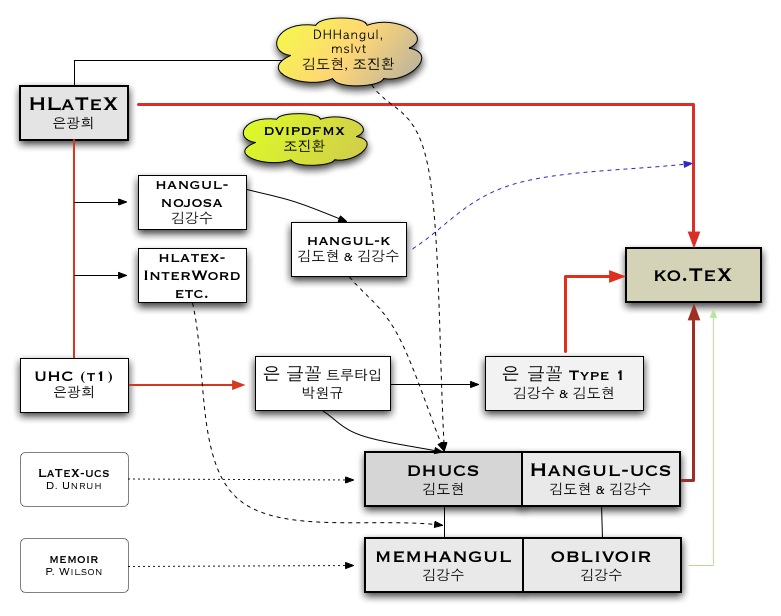
\includegraphics[width=\linewidth]{kotexhist}
\caption{\protect\kotex 의 탄생}\label{fig:hist}
\end{figure}

그림~\ref{fig:hist}\는 H\LaTeX 에서 출발하여 \kotex 에 이르는
한글 텍의 발전 과정을 요약한 것이다. 

2007년 6월 30일, 한국텍학회 모임에서, 은광희\cntrdot 김도현\cntrdot 김강수 등
한글 라텍\cntrdot hangul-ucs의 저자들과 KTS 임원\cntrdot 회원 등이 모인 자리에서
이 두 한글 매크로 패키지를 통합하여 \wi{통합 한글 텍 패키지}를 제작하기로
의견을 모은 것이다. 이것은 그 동안 한글 사용에 있어서 둘 이상의 패키지가
존재함으로 인해 빚어진 혼란을 불식하고 향후 한글 텍/라텍의 발전의
근거를 마련했다는 점에서도 중요한 일보전진이었고, 한글 라텍으로부터
오랜 시간 발전해 온 라텍에서의 한글 사용을 총체적으로 점검할 기회를
얻게 되었다는 점에서도 의미가 있는 결정이었다.

그로부터 일 개월 정도의 작업을 통하여 \kotex\ 베타 버전이 공개되었다.
\kotex 은 Unicode/UTF-8 인코딩과 EUC-KR을 모두 지원하기로 하였으나
원칙적으로 향후의 발전 방향은 Unicode로 합의하였다. 또한 은광희의
UHC 글꼴을 발전시킨 `은 글꼴 type 1'을 기본 글꼴로 채택하고 이를
EUC-KR 버전에도 적용시킴으로써, 폰트를 둘러싼 이런저런 불편한 점을
일소하였으며, pdf 제작 및 매크로의 호환성과 안정성에 있어서
몇 가지 중요한 진보를 이루었다.


\chapter{설치}\index{설치}

\section{\TeX\ 배포판}

각 플랫폼별로 유명한 \TeX\ 배포판\footnote{%
  \TeX~implementations}%
들이 있다. 리눅스에서는 Thomas Esser의 te\TeX 이 부동의 지위를 오랜 동안
지켜왔으며,
매킨토시에서는 Classic Mac 시기의 Oz\TeX 이 퇴조하고 Mac OS X 하에서
Gerben Wierda의 gw\TeX 이 널리 쓰였다. 
윈도우즈는 사정이 복잡하지만 MiK\TeX 이 사실상 가장 많은 사용자를 가진
시스템이 되었으나 Fabrice Popineau의 fp\TeX 도 한동안 유수한
사용자를 보유하고 있었다. MiK\TeX 을 제외하면 이 모두가 web2c에서
파생된 시스템이라는 공통점을 지니고 있다. MiK\TeX 도 종래에는
web2c를 변형해서나마 받아들이게 되었다. 

그런데 2007년에 접어들면서 사정이 일변한다. 우선 te\TeX 과
gw\TeX 의 개발이 중단되었다. 또한 web2c 역시 독자적인 배포판(소스)로서
유지되지 않게 되었다. 그 대안으로 \TeX{}Live가 새로운 표준으로
등장했기 때문이다.

윈도우즈의 경우, 사정은 더욱 복잡해졌다. KTUG에서는 2006년, \TeX{}Live와
무관하게 독자적인 배포판 KTUG Collection을 제작하였는데, 이것은
web2c로부터 파생된 Akira Kakuto의 W32TeX의 바이너리를 가져다 쓴
것이었다. 다행히도 \TeX{}Live 자체가 W32TeX을 채택함으로써,
KC2006과 \TeX{}Live는 그 차이가 미미한 대단히 유사한 시스템이
되었다.\footnote{%
  내부적으로 차이점은 많다. 특히 한글 운영에 필요한 다양한
  유틸리티를 제공하는 것, 일괄 인스톨러를 제공하는 것, 패키지
  관리 유틸리티와 업데이트 유틸리티를 제공하는 것, 셸 유틸리티(KCmenu)를
  제공하는 것 등은 \TeX{}Live보다 KC2006을 더욱 편리한 시스템이
  되게 한 면이 있다.}
  
이 글은 \TeX{}Live 2007을 기준으로 작성한다. 
매킨토시와 리눅스 등 유닉스-류 운영체제에서는 \TeX{}Live 이외의 대안이
현재로서는 없다. 일부 리눅스 시스템에서 te\TeX 이 여전히 주류를 이루고
있으나 조만간 \TeX{}Live로 이행하게 되리라고 기대한다.
\TeX{}Live는 방대하기도 하거니와 대단히 안정적으로 동작하는
시스템으로, 사실상 다양한 배포판의 시대를 종결시킨 `유일' 배포판의
지위를 차지할 것으로 예측된다.\footnote{%
  MiK\TeX 에 대하여 별도로 언급하지 못하는 것은 유감이다.
  그러나 MiK\TeX~사용자들은 MiK\TeX 에서 \kotex 을
  설치하는 적절한 방법을 찾아낼 것이라고 믿는다.}

일부 상업용 \TeX{} 배포판의 경우는, 그 배포판을 판매하는 측에서
한글 사용에 관한 해결책을 제시하는 것이 옳다고 생각한다. 이 글은 상업용 배포판에 대해서는
별도의 언급을 할 수 없을 것이다.

\section{\protect\eTeX}

\kotex/utf는 \eTeX 을 요구한다. \eTeX 의 확장 프리미티브를
활용하고 있기 때문이다. \pkg{kotexplain}도 \texttt{tex}으로는
컴파일되지 않으며 \texttt{etex}이나 \texttt{pdftex}을 이용하여야
한다.

다행히 \TeX{}Live 2007에서 \texttt{latex}은 \eTeX{} 엔진을
사용하도록 조성되어 있는 것이 기본값이므로 \LaTeX{} 사용에
있어서 사용자가 별달리 주의할 것은 없다. 

다른 \TeX{} 배포판, 예컨대 te\TeX{} 등에서는 \texttt{elatex}이나
\texttt{pdfelatex}을
실행하지 않으면 안되는 경우도 있을 수 있다. 텍 시스템의 기본
\LaTeX{} 엔진을 \eTeX 으로 바꾸는 것은 쉽게 할 수 있으나
이 글의 범위를 넘어선다. 

\section{디렉터리 구조(TDS)}\index{TDS}

표준적인 web2c 시스템(\TeX{}Live는 web2c 시스템이다)에서는
방대한 파일을 간단하게 찾기 위해서 kpathsearch라는 라이브러리를
이용한다. kpathsearch 라이브러리는 필요한 파일들이 일정한 디렉터리
구조에 따라 배치되어 있다고 가정하기 때문에 \TeX{} 시스템에서
파일은 이러한 디렉터리 구조(TDS\footnote{%
  TeX Directory Structure. \url{http://www.tug.org/tds/tds.pdf}})를
따라 배치되어 있어야 한다. 이 글에서는 2004년 발표된
TDS version 1.1을 기반으로 설명한다.\footnote{%
  MiK\TeX~2.6은 TDS 1.1을 잘 따르지 않는 것으로 알려져
  있다. 그러므로 아래의 설명은 MiK\TeX 에 적용되지 않는다.}

이 규정에 따르면, 텍에 필요한 파일들은 TDS의 출발점인 \texttt{TEXMF}
밑에 두게 된다.
\texttt{TEXMF}는 텍의 원천 코드를 컴파일할 때
결정되며, 둘 이상을 둘 수 있다. \TeX{}Live는 \texttt{texmf,
texmf-dist, texmf-doc}라는 기본 \texttt{TEXMF} 트리와 더불어
사용자가 설정할 수 있는 \texttt{texmf-local, \$HOME/texmf} 등을
사용한다. 이들을 편의상 \texttt{TEXMF} root라고 부르기로 하겠다.

한 시스템에 여러 사용자가 있을 때, 시스템 전체에 적용되는 \texttt{TEXMF}들과
개별 사용자 자신이 이용하는 \texttt{TEXMF}도 분리할 수 있다. 
이미 설치된 텍 운영 체계에서도 \texttt{texmf.cnf} 파일에서
\texttt{TEXMF}를 다시 설정할 수 있다.  TDS를 준수할 경우, 서로 다른
텍 배포판에서도 \texttt{TEXMF} root의 경로만 다를 뿐이고 그
이하의 디렉터리 구조는 같다.

\kotex 은 위의 어떤 \texttt{TEXMF} root 아래 설치되어도 무방하다.
이 위치를 편의상 \texttt{[texmf]}라고 표시하겠다. 
예컨대 \texttt{/usr/local/texlive/texmf-local}을 \kotex 이
설치될 위치로 선정할 수 있을 것이다. 되도록이면 \texttt{.../texlive/2007/texmf}이나, \texttt{texmf-dist}와 같은 시스템 디렉터리와는 분리하는 것이
좋다. 

`\texttt{Top-level directories}'는 텍 운영 체계의 구성 요소로서 \texttt{tex} (텍
파일), \texttt{fonts} (폰트 관련 파일), \texttt{metafont} (폰트가 아닌
\MF{} 파일), \texttt{metapost} (\MP{} 파일), \texttt{bibtex}(Bib\TeX{}
파일), \texttt{scripts} (운영 체계 독립적인 실행 파일), \texttt{doc}
(사용자용 문서 파일), \texttt{source} (원천 파일), \texttt{<구현>}
(\texttt{emtex, vtex, web2c}와 같은 텍 구현 관련 파일),
\texttt{<프로그램>} (\texttt{mft, dvips}와 같은 프로그램에 따른 입력 및
설정 파일) 등등이 해당된다.

텍 체계를 구성하는 모듬 명령(매크로) 파일의 위치는 다음과 같은 계층 구조를
갖는다.
\begin{verbatim}
        TEXMF/tex/틀/꾸러미
\end{verbatim}

`\texttt{틀}'은 텍의 용어로 \verb|\dump| 되는 것들을 말하는데,
\kotex 은 플레인텍(plain\-\TeX)을 위한 kotexplain, 라텍을 위한 \kotex-euc/utf
등으로 이루어지므로, 거기에 맞게 \texttt{[texmf]/tex/plain/kotex} 
또는 \texttt{[texmf]/tex/latex/kotex} 등의 위치에 놓이게 된다.

글자체는 다음과 같은 규정에 의해 설치할 것을 요구한다.
\begin{verbatim}
        TEXMF/fonts/형식/제공자/글자체
        TEXMF/fonts/{enc,lig,map}/하위경로
\end{verbatim}
`\texttt{형식}'은 글자체의 종류를 가리킨다.  즉, 
\texttt{tfm}, \texttt{vf}, \texttt{type1},
\texttt{afm} 등이 이에 해당한다.  글자체의 부호화나 합자 혹은 글자체
이름 대응 파일들은 각각 \texttt{enc, lig, map} `\texttt{형식}' 디렉터리에
평행한 디렉터리에 따로 둔다.  `\texttt{제공자}'의 대상은 글자체를
만드는 업체나 만든이 등인데,  adobe 회사의 type 1 글자체
(\texttt{adobe}), bitstream 회사의 type 1 글자체 (\texttt{bitstrea}),
D.~Knuth 교수의 \MF{} 글자체 (\texttt{public}), J.~Knappen 씨의 \MF{}
글자체 (\texttt{jknappen}) 등을 예로 들 수 있다.
`\texttt{글자체}'는 글자의
모양에 따른 이름이다.  adobe 회사에서 만든 글자체에는
\texttt{times}, \texttt{helvetic} 등의 이름이 사용되고 D.~Knuth 교수가
텍 운영 체계를 위해서 만든 글자체의 경우는 \texttt{cm}, \texttt{ec}
등의 이름이 사용되며 \kotex 에서 제공하는 글자체에서는
\texttt{myoungjo}, \texttt{gothic} 등의 이름이 사용된다.

\kotex 의 글자체들은 다음처럼 위치하게 된다.
\begin{verbatim}
    [texmf]/fonts/형식/kotex/{base,extra}/{myoungjo,gothic,...}
    [texmf]/fonts/map/dvips/kotex
\end{verbatim}


\section{일반적인 설치 지침}

\subsection{다운로드}\label{sec:download}

\url{ftp://ftp.ktug.or.kr/KTUG/ko.TeX/} 디렉터리에서 배포되는
압축 파일은 다음 두 개이다.
\begin{itemize}
\item \href{http://ftp.ktug.or.kr/KTUG/ko.tex/ko.tex-macro.tar.gz}{ko.tex-macro.tar.gz}
\item \href{http://ftp.ktug.or.kr/KTUG/ko.tex/ko.tex-unfonts-base.tar.gz}{ko.tex-unfonts-base.tar.gz}
\end{itemize}
둘 다 \texttt{.tar.gz}로 압축된 파일로서 gunzip과 tar를 이용하여
압축해제할 수 있다. 

\subsection{매크로와 유틸리티}
먼저 \texttt{*-macro-*} 압축파일을 적당한 곳에 풀면, 몇 개의 파일(INSTALL,
LICENSE 등)과 일곱 개의 하위 디렉터리를 얻을 수 있다. 이것을 다음과 같이
이동한다.
\begin{verbatim}
================================================================
 subdirectories and/or files    destination
================================================================
 bibtex/euc                     [texmf]/bibtex/bst/kotex/euc
 doc/*                          [texmf]/doc/latex/kotex/*
 latex/*                        [texmf]/tex/latex/kotex/*
 makeindex/*                    [texmf]/makeindex/kotex/*
 plain/*                        [texmf]/tex/plain/kotex/*
 sfd/*                          [texmf]/fonts/sfd/*
 util/*.pl                      [texmf]/scripts/kotex/perl/*.pl
================================================================
\end{verbatim}

\texttt{util} 디렉터리 안에는 두 개의 \texttt{.c} 소스와 몇 개의
\texttt{*.pl} 스크립트가 있다. 이 중 \texttt{.c}는 컴파일하고\footnote{%
  윈도우즈용으로 \texttt{.exe} 파일이 함께 제공된다.}
\texttt{*.pl}은 실행 권한을 부여하여 \texttt{/usr/local/bin/}으로
이동한다.\footnote{%
  윈도우즈에서는 Active Perl 등을 설치하여 이 스크립트를 실행 가능하게 
  해두어야 한다. 혹은 설치 패키지를 이용하는 경우 \texttt{.exe} 형식
  파일로 제공하는 경우도 있을 것이다.}
\begin{verbatim}
hbibtex.c
  $ gcc -o hbibtex hbibtex.c
  $ cp ./hbibtex /usr/local/bin/
hmakeindex.c
  $ gcc -o hmakeindex hmakeindex.c
  $ cp ./hmakeindex /usr/local/bin/
*.pl
  $ chmod a+x *.pl
  $ cp ./*.pl /usr/local/bin/
\end{verbatim}


\subsection{글자체의 설치}

\texttt{*-fonts-base-*} 압축 파일을 내려받은 다음 적당한 곳에 풀면
라이센스 관련 파일 몇 개와 함께 두 개의 하위 디렉터리가 있다. 이것을
아래와 같이 이동한다.
기본으로 배포되는 폰트 패키지에는 명조, 고딕, 타자, 그래픽, 네 글꼴 가족만
포함되어 있다. 이밖의 `은 글꼴' 시리즈는 extra 폰트라는 이름으로 배포되는데,
만약 많은 글자체를 필요로 한다면 extra 패키지까지 설치해야 할 것이다.
설치 방법은 동일하다. 
\begin{verbatim}
========================================================
 directory                   destination
========================================================
 fonts                       [texmf]/fonts
 tex                         [texmf]/tex
========================================================
\end{verbatim}

이 글자체들에 대한 정보를 텍 엔진에게 알려주는 것이 updmap을 통한
map의 생성이다. \TeX{}Live 2007은 이 과정을 매우 간편하게 진행할
수 있는데, 다음 절차를 따르면 된다.
\begin{verbatim}
$ mktexlsr
$ updmap-sys --enable Map=kotex-base.map
\end{verbatim}
만약 super user 권한을 가지고 있지 않다면 \texttt{updmap-sys} 대신
\texttt{updmap}을 실행한다. 

extra 폰트 패키지도 설치했다면
\begin{verbatim}
# mktexlsr
# updmap-sys --enable Map=kotex-extra.map
\end{verbatim}
이것으로 끝이다.

\section{각 플랫폼별 설치 패키지}

앞 절에서 설명한 일반적 설치 지침을 따르는 것이 번거롭고 불편할 수도 
있으므로 그럴 때는 간편한 각 배포판, 플랫폼별 설치 패키지를 이용하는
방법이 있다. \href{http://ftp.ktug.or.kr/KTUG/ko.TeX/instpack/}{install
package}\footnote{\url{http://ftp.ktug.or.kr/KTUG/ko.TeX/instpack/}} 디렉터리에 가면 윈도우즈 KC2006 및 매킨토시 \TeX{}Live를 위한
설치 패키지가 마련되어 있다. 리눅스는 각 배포판별로 간편한 설치
유틸리티를 제작할 수 있을 것인데, 이에 대한 정보는 \href{http://faq.ktug.or.kr/faq/ko.TeX/instpack}{KTUGFaq::ko.TeX/instpack} 페이지\footnote{\url{http://faq.ktug.or.kr/faq/ko.TeX/instpack}}에서
찾을 수 있다.

\section{CVS 개발 버전}

\href{http://cvs.ktug.or.kr/viewcvs/ko.TeX/}{CVS::ko.TeX}\footnote{%
  \url{http://cvs.ktug.or.kr/viewcvs/ko.TeX}}%
에서
최신의 개발 버전을 확인할 수 있다. \ref{sec:download} 절에서 언급한
파일들은 CVS snapshot을 정기적으로 릴리스한 것이므로 비교적 안정적이나,
CVS 개발 버전은 사용자가 개발에 참여할 의사가 있거나 최신 버전을 활용하고자 할 
때, cvs를 통하여 다운로드받을 수 있을 것이다. 

anonymous로 CVS를 리트리브하려면 다음과 같이 한다.
\begin{verbatim}
$ cvs -d :pserver:anonymous@cvs.ktug.or.kr:/home/cvsroot login
$ cvs -d :pserver:anonymous@cvs.ktug.or.kr:/home/cvsroot \
  checkout ko.TeX
\end{verbatim}
패스워드를 물어오면 그냥 엔터를 치면 진행할 수 있다.

\chapter{사용}

한글 라텍 \kotex 은 은광희의 H\LaTeX 과 김도현\cntrdot 김강수의 hangul-ucs를 
합쳐서 하나의 패키지로 구성한 것이다. 1990년대 이래 한글 사용의 사실상
표준이었던 이 두 패키지가 결합함으로써 명실공히 라텍에서의 한글 사용에
새로운 장을 열었다고 평가해도 좋으리라.

\kotex 은 본격적인 한국어(한글) 텍 시스템이다.\footnote{\kotex은 텍스트
  상황에서 \texttt{ko.TeX}이라고 쓰고 ``케이오텍'' 또는
  ``코리언 텍''이라고 읽는다. \texttt{ko}는 한국어를 의미하는
  국제부호에서 취한 것이다. \texttt{ko}를 소문자로 쓴다.}
라텍은 물론이고 플레인텍에서 컨텍스트에
이르기까지 거의 모든 텍 관련 매크로에서 한글을 구현하도록 할 수 있다.
그래도 그 중심은 역시 한글 `라텍'일 것이다. 
이 글은 한글 `라텍'에 대해서 주로 다루고 다른 매크로에서의 한글 구현에
관한 사항은 별도의 장으로 설명하겠다. 앞으로 별다른 언급이 없으면 \kotex 이
한글 라텍 매크로를 (주로) 가리키는 것으로 하자.

한글 라텍으로서 \kotex 은
EUC-KR 코드와 UTF-8 한글 코드를 지원한다.\footnote{%
  윈도우즈에 친숙한 CP949 코드는 지원하지 않는다. CP949는 사실상
  유니코드의 현대 한글 음절 영역에서 다룰 수 있는 모든 문자에
  해당하므로 유니코드를 통하여 지원하는 것이 바람직하다고 판단하였다.}
그 가운데 EUC-KR 지원은 일종의 ``하위호환성'' 측면에서 제공되는 것으로,
향후 발전은 UTF-8 부분만 반영될 것이다. EUC-KR 코드로 작성된 기존의 한글 문서를
컴파일할 수 있고 이것을 더 쉽게 UTF-8 문서로 바꿀 수 있게 하는 것이
두 코드를 모두 지원하는 원래의 목적이며 EUC-KR 버전은 UTF-8 버전과
항상 동일하게 동작하지 않는다. 또한 EUC-KR 한글 문서는 비교적 쉽게
UTF-8로 포팅할 수 있으나 그 역의 경우는 잘 되지 않거나 많은 노력이
필요할 수 있다. 

그럼에도 불구하고 \kotex/euc는 H\LaTeX 에 비해서 다음과 같은 점이 개선되었다. 주로 pdf 제작과 관련된 것들이 많다. \euc
\begin{enumerate}
\item
pdf 책갈피를 만들어도 한글이 ``깨지지'' 않게 할 수 있다.
\item
pdf 문서에서 한글 텍스트의 검색과 추출이 되게 할 수 있다.
\item
KTUG에서 발전한 한글 타이포그래피의 성과를 부분적으로나마 이용하여 비교적 잘 정돈된 한글 문서를 만들어낸다. 
그러나 utf 버전은 더욱 발전된 타이포그래피를 다루고 있으므로 되도록이면 utf 버전이 사용되기를 희망한다. 
\end{enumerate}

한편, hangul-ucs에 비해서는 주로 (linux에서의) 설치와 관련된 문제가 현저히 개선되었다. \utf
\begin{enumerate}
\item
latex-ucs 패키지에의 의존성이 없다.
\item
ttf2pk를 사용하지 않음으로써 ttf2pk에 대한 의존성도 사라졌다.
\item
H\LaTeX 과 통합되었으므로 hlatex에 대한 의존성도 필요없다.
\item
트루타입 `은 글꼴'을 사용하지 않기 때문에 별도로 폰트를 설치해야 하는 불편이 없다.
\item
dvipdfmx.cfg나 ttf2pk.cfg 등의 설정 파일 수정을 일일이 해야 하는
불편이 없어지고 updmap에 의한 일괄 명령 한 번으로 모든 폰트 설정이 이루어진다.
\item
기본 패키지의 크기가 이전에 비하여 현저히 줄었다.
\end{enumerate}

\section{기본 사용법}

\kotex 의 기본 스타일은 \texttt{kotex.sty}이다. 다음과 같이 쓴다.
\begin{verbatim}
\usepackage{kotex}
\end{verbatim}

\utfeuc 언어 코드를 첫번째 인자로 지정하는데, 디폴트는 utf이다. 그러므로 utf는
별도로 명시하지 않아도 되지만 euc 문서를 작성할 때는 반드시 euc 옵션을
되도록 맨처음에 지정한다.
\begin{verbatim}
\usepackage[euc]{kotex}
\end{verbatim}

\begin{center}
\begin{ttfamily}
\begin{tabular}{l|l}
\hline
명령 & 대응 \\ \hline
\bs usepackage\{kotex\} & \bs usepackage\{dhucs\} \\
\bs usepackage[hangul]\{kotex\} & \bs usepackage[hangul]\{dhucs\} \\
\bs usepackage[euc]\{kotex\} & \bs usepackage\{hfont\} \\
\bs usepackage[euc,hangul]\{kotex\} & \bs usepackage\{hangul\} \\
\hline
\end{tabular}
\end{ttfamily}
\end{center}

H\LaTeX 에는 두 가지 사용법이 있었다. 하나는 \texttt{hfont}이고 다른
하나는 \texttt{hangul}이었다. \kotex 에서는 한글 서식 hangul 옵션이
주어진 상태와 그렇지 않은 상태로 구분한다. 영문 위주 문서에 한글을 
사용할 때는 hangul 옵션 없이 쓰고, 한글 위주의 문서에서 한글식 서식을
설정하려면 hangul 옵션을 지정한다.

\paragraph{kotex.cfg} 사용자는 일반적으로 utf나 euc 가운데 한 가지를
주로 쓰지 둘 다 쓰게 되는 경우는 거의 없을 것이다. kotex.cfg 파일은 
이럴 경우에 대비하여 자신이 쓰는 kotex 옵션을 미리 지정해두고 단순히
\verb|\usepackage{kotex}|이라고만 하여 그 옵션들을 활성화하게 할
수 있다. 이 파일은 \texttt{[texmf-ktug]/tex/latex/kotex/}에
있으므로 자신에게 맞게 적절하게 수정해서 쓰도록 한다. 

\section{pdf 문서 작성을 위한 설정}\label{sec:makepdf}

\subsection{\kotex/utf 문서}
\utf utf 문서는 다음과 같이 한다. 유니코드 문서에서는 hyperref에
\texttt{[unicode]} 옵션을 지정하는 것으로 pdf bookmark 문제가
모두 해결되므로, .out 파일의 코드 변환과 같은 문제에 신경쓸 필요가
없다.
\begin{verbatim}
\usepackage{kotex}
\usepackage{ifpdf}
\newcommand\myDRIVER{\ifpdf pdftex\else dvipdfm\fi}
\usepackage{\myDRIVER,unicode,bookmarks]{hyperref}
\end{verbatim}
여기서는 [unicode] 옵션이 반드시 지정되어야 한다. 그리고 CJKbookmarks를
쓰지 않는 점이 다르다. 또한 euc-bookmark와 같은 번거로운 절차가
필요없다. 위의 예에 상당하는 컴파일 절차 예시는 다음과 같다.\footnote{%
  \texttt{komkindex}는 Perl Script이므로 경우에 따라
  \texttt{komkindex.pl}을 실행해야 할 것이다. 이후로도 같다.}
\begin{verbatim}
$ (pdf)latex foo
$ bibtex foo
$ komkindex -s kotex foo
$ (pdf)latex foo
$ (dvipdfmx foo)
\end{verbatim}

pdf 문서의 텍스트 검색과 추출은 매우 중요한 문제이다.
이것은 어떤 드라이버로 pdf를 생성하느냐에 따라 조금 달라지는데, 일괄
요약하면 다음과 같다.
\begin{description}
\item[dvipdfmx] 기본 폰트인 type 1 글꼴을 매우 잘 처리하고
이로부터 검색 및 추출이 가능한 pdf를 만들어낸다. 별도의 조치가
필요없다.
\item[dvips] 트루타입을 처리하지 못하는 점 때문에 이전부터
문제가 있다고 생각되었으나 적어도 \kotex 이 제공하는 폰트를 사용하는 한
검색 추출에 문제는 없다. 역시 별도의 조치가 필요없다.
\item[pdf\TeX] 이 때는 \texttt{\bs pdfgentounicode}를
활성화해주어야 한다.
\end{description}
그러므로, preamble에 다음과 같이 선언하는 것으로 될 것이다.
\begin{verbatim}
\ifpdf
  \input glyphtounicode
  \pdfgentounicode=1
\fi
\end{verbatim}

어떤 드라이버를 사용하든 모두 포스트스크립트 윤곽선 글꼴이 사용되고,
pdf 북마크가 잘 만들어져 있으며 한글 텍스트의 검색 및 추출이 자유롭다.


\subsection{\kotex/euc 문서}

\euc\begin{verbatim}
\usepackage[euc]{kotex}
\usepackage{ifpdf}
\newcommand\myDRIVER{\ifpdf pdftex\else dvipdfm\fi}
\usepackage[\myDRIVER,CJKbookmarks]{hyperref}
\end{verbatim}

위의 것은 euc 문서를 위한 설정이다. \texttt{hyperref}는 거의 필수이므로
이를 로드하여야 하고, 북마크는 \texttt{CJKbookmarks} 옵션을 준다. 
이제 이 문서를 처리하는 과정에서, 맨 마지막 \LaTeX{} 컴파일
직전에 euc-bookmark 유틸리티를 한번 실행해주면 된다. 이 유틸리티가
하는 일은 북마크를 위한 파일의 인코딩을 hyperref가 이해하는 유니코드
인코딩으로 바꾸어주는 일이다. 그러므로 컴파일 과정을 예시하면 다음과 같이
될 것이다.\footnote{%
  KC2006을 위한 설치 패키지에서는 komkindex.exe 등을
  제공하기도 한다. 이 때는 굳이 \texttt{.pl}과 같은
  확장명을 붙이지 않아도 된다. 또한 \texttt{cp} 명령은
  윈도우즈에서는 \texttt{copy}이다.}

\begin{verbatim}
$ pdflatex foo
$ hbibtex foo
$ komkindex -euc -s hind foo
$ euc-bookmark.pl foo.out >foo-a.out
$ cp foo-a.out foo.out
$ pdflatex foo
\end{verbatim}

DVIPDFM$x$를 이용하려 하는 경우 불편한 euc-bookmark를 쓰지 않아도
한글 북마크를 잘 만들어준다. 이 때는 다음과 같은 코드가 필요하다.
\begin{verbatim}
\ifpdf\else
 \AtBeginDvi{\special{pdf: tounicode KSCms-UHC-UCS2}}
\fi
\end{verbatim}
그리고 다음 순서로 컴파일하면 된다.
\begin{verbatim}
$ latex foo
$ hbibtex foo
$ komkindex -euc -s hind foo
$ latex foo
$ dvipdfmx foo
\end{verbatim}
이것은 오직 DVIPDFM$x$를 쓰는 경우에만 유효하다.

\subsection{요약}

이상을 요약하면, 다음과 같다.

\bigskip
\noindent\uline{UTF:}
\begin{verbatim}
\documentclass{article}
\usepackage{kotex}
\usepackage{ifpdf}
\ifpdf
  \usepackage[unicode]{hyperref}
  \input glyphtounicode\pdfgentounicode=1
\else
  \usepackage[unicode,dvipdfm]{hyperref}
\fi
\end{verbatim}
\medskip
\noindent\uline{EUC:}
\begin{verbatim}
\documentclass{article}
\usepackage[euc]{kotex}
\usepackage{ifpdf}
\ifpdf
  \usepackage[CJKbookmarks]{hyperref}
  \input glyphtounicode\pdfgentounicode=1
\else
  \usepackage[dvipdfm,CJKbookmarks]{hyperref}
  \AtBeginDvi{\special{pdf: tounicode KSCms-UHC-UCS2}}
\fi
\end{verbatim}

이와 관련하여 다음 두 가지를 지적해 두기로 한다.
\begin{enumerate}
\item 위의 코드가 제대로 동작하려면 KSCms-UHC-UCS2라는 이름의
cmap이 있어야 한다. 이 cmap은 ghostscript의 resource 디렉터리에
들어 있으므로, 만약 cmap을 찾는 데 실패하는 에러를 만난다면
자신의 \TeX\ 시스템에게 이 cmap 위치를 알려주도록 하라.
\item 위의 \texttt{pdfgentounicode}에 관련된 것은 type 1 글꼴이
사용되었을 때 유효하다. 사용자가 자신의 개인적인 용도로 트루타입으로
조판하려 한다면 이 코드보다는 \verb|\usepackage{dhucs-cmap}|을
선언하도록 하여야 한다.
\end{enumerate}

\section{폰트에 대하여}\label{sec:aboutfont}

\kotex 의 가장 큰 특징이 폰트에 관련된 부분이다. 기본 글꼴로
``은 글꼴 type 1''을 채택하였는데 이것은 H\LaTeX 의
기본 글꼴이었던 UHC 글꼴을 트루타입으로
바꾼 은 글꼴(hangul-ucs의 기본 글꼴)로부터 얻어진 type 1이다. 

원래 UHC 글꼴이 type 1이었는데 왜 은 글꼴로부터 별도로 type 1 글꼴을
만들어내어야 했던가? 그것은 UHC 글꼴이 가진 독특한 특성, 즉 자소 글꼴이라는
점 때문이었다. UHC 폰트 자체는 일종의 자소 글꼴로서, 이것을 실제의
문자에 대응시키기 위해서는 vf를 통하여 자소 조합을 실행해야 한다.
각 문자에 유니코드 코드 포인트를 대응시켜주어야 텍스트의 검색 추출이
가능해질 것이므로 UHC 폰트 자체만으로는 이것을 하는 것이 어려웠다.
반면 은 글꼴 type 1은 유니코드 배열에 따라 완성된 문자를 가지고 있는
글꼴이다. 은 글꼴 type 1 자체가 UHC에 기원을 두고 있으니만치, 
``은 글꼴 type 1은 UHC의 자소를 미리 조합하여 유니코드 코드 포인트를
부여한 글꼴''이라고 이해할 수 있으리라 생각한다. 

\begin{center}
\fbox{%
UHC 글꼴 (H\LaTeX) $\longrightarrow$
은 글꼴 (hangul-ucs) $\longrightarrow$
은 글꼴 type 1 (\kotex)
}
\end{center}

\subsection{기본 글꼴}

기본(base) 폰트는 명조(바탕), 돋움(고딕), 타자, 굴림의 네 종류이다. 

\begin{center}
\begin{tabular}{lcccccc}
\hline
글꼴 & file & name(utf) & name(euc) & 한자 & 볼드 & 변형(c,o)\\ \hline
명조 & outbtmXX & utbt & mj (wmj) & O & O & O \\
고딕 & outgtmXX & utgt & gt (wgt) & O & O & O \\
타자 & outtzmXX & uttz & tz (wtt) & X\footnotemark & X & X \\
그래픽 & outgrmXX & utgr & gr (wgr) & X & O & O \\
\hline
\end{tabular}
\footnotetext{고딕의 한자를 가져다 쓴다.}
\end{center}

euc와 utf 양쪽에서 모두 동일한 글꼴을 사용하는데, 다만 euc에서는
vf를 통하여 필요한 글자를 뽑아서 완성형 인코딩에 맞게 재배열하여
사용한다.

\subsection{추가 글꼴} 

추가 폰트(extra)에는 은 글꼴의 나머지 폰트들이 들어 있다. 한자 등이
들어 있거나 변형 글꼴이 제공되는 것은 다음과 같다. 

\begin{center}
\begin{tabular}{lcccccc}
\hline
글꼴 & file & name(utf) & name(euc) & 한자 & 볼드 & 변형(c,o) \\ \hline
신문 & outshmXX & utsh & sh (wsh) & O & X & O  \\
옛글 & outytmXX & utyt & yt (wyt) & O & X & O \\
궁서 & outgsmXX & utgs & gs (wgs) & O & X & O \\
필기 & outpgmXX & utpg & pg (wpg) & X & O & O \\
봄 & outbmmXX & utbm & bm (wbm) & X & X & O \\
\hline
\end{tabular}
\end{center}

다음 추가 글꼴은 굵은 글꼴, 기울인 글꼴, 장평줄인 글꼴 등의 변형 서체를
전혀 지원하지 않고 오직 기본 모양 하나만으로 제작된 것들이다.

\begin{center}
\begin{tabular}{lcccccc}
\hline
글꼴 & file & name(utf) & name(euc) & 한자 & 볼드 & 변형(c,o) \\ \hline
자모명조 & outjbtmXX & utjbt & jbt & X & X & X \\
자모고딕 & outjgtmXX & utjgt & jgt & X & X & X \\
자모노벨 & outjnvmXX & utjnv & jnv & X & X & X \\
자모소라 & outjsrmXX & utjsr & jsr & X & X & X \\
펜글씨 & outpnmXX & utpn & pn & X & X & X \\
펜흘림 & outphmXX & utph & ph & X & X & X \\
\hline
\end{tabular}
\end{center}

이상 15종의 폰트가 트루타입 은 글꼴 시리즈에 대응한다. 여기에 H\LaTeX{}
1.0에서 새로 도입된 세 종류 글꼴 중 두 종류를 추가 글꼴(extra-hl)로
제공한다. 이 추가글꼴들도 기울임/장평줄임 등의 변형 글꼴 없이(즉,
m-시리즈만으로) 제공된다. 

\begin{center}
\begin{tabular}{lcccccc}
\hline
글꼴 & file & name(utf) & name(euc) & 한자 & 볼드 & 변형(c,o) \\ \hline
디나루 & outdnmXX & utdn & dn (wdn) & X & O & X \\
필기a & outpgamXX & utpga & pga & X & X & X \\
\hline
\end{tabular}
\end{center}
\euc 참고로, euc에서 extra-hl 폰트를 사용하려면 \verb|\usepackage{extra-hlfont}|를
지시해주어야 한다. 

각 폰트의 인쇄된 모양을 보려면 부록을 참고하라.

\subsection{은 글꼴 트루타입 폰트 세트}

hangul-ucs에서 사용하던 은 글꼴 트루타입 폰트도 사용이 가능하다.
이것은 별도로 설치를 하여야 하며, 은 글꼴 트루타입도 별도로
시스템에 등록하여야 한다.

\utf utf에서는 일반적인 방법으로 이 폰트를 사용할 수 있다. 다만
폰트 명칭이 \texttt{ut..}가 아니라 \texttt{un..}이라는 점을 알아두자.
따라서 예컨대 \\
\verb|  \SetHangulFonts{unbt}{ungt}{untz}|\\
\verb|  \SetHanjaFonts{unbt}{ungt}{ungtz}|\\
와 같이 선언하여 은 글꼴 트루타입을 쓰도록 할 수 있다.

\euc euc에서 은 글꼴 트루타입을 쓰려면 \verb|\usepackage{unttf}|를
선언한다.

트루타입 사용은 DVIPDFM$x$로 pdf를 제작할 때 유용하다. pdf\TeX 에서
사용하지 못하는 바는 아니지만 기울인 글꼴 등이 잘 처리되지 않는다. 
은 글꼴 type 1과 은 글꼴 트루타입은 사실상 같은 글꼴이라고 보아도 무방하다.

\subsection{타자 글꼴에 관한 주석}

은타자는 현재 거의 유일한 고정폭(monospaced) 글꼴이다. 이 글꼴에
대해서 그 디자인을 두고 논란이 없는 것은 아니지만 그래도 \verb|\ttfamily|에
대응하는 고정폭 글꼴의 필요성을 고려한다면 매우 중요한 글꼴이라고 할 수 있다.

고정폭으로 쓰일 것이므로 볼드나 기울임 등은 불필요하다. 또한 폭을 변경시키는
변경폭(c-시리즈, x-시리즈)도 제공될 필요가 없다. 타자 글꼴 자체에 한자가
들어 있지 않은데, \kotex 의 타자 글꼴은 \texttt{uttz}로 지정해도
가상 글꼴을 통해 고딕(돋움)의 한자 부분을 타자체의 폭에 맞게 조절하여
사용한다. 은 글꼴 트루타입은 그렇지 않으므로 위의 예와 같이 \texttt{ungtz}로
해야 한다.

\subsection{요약}

\kotex 은 ``은 글꼴 type 1''을 기본 폰트로 한다.

이로부터 얻을 수 있는 이점은 다음과 같다.
\begin{enumerate}
\item
pdf\TeX 에 친화적인 폰트 세트이다. pdf\TeX 과 DVIPDFM$x$, 심지어
dvips까지 모두 이 형식의 폰트를 잘 다루므로 범용성과 호환성이 매우
높아졌다. pstricks를 위해서 폰트를 바꾸어야 하는 불편을 없앴다.
\item
\TeX{} 배포판의 유용한 유틸리티 updmap을 이용하여 설치하므로 설치
과정이 깔끔하게 끝난다.
\item
pdf\TeX, DVPIDFM$x$, dvips 어떤 것으로도 한글 텍스트의 검색과
추출이 되는 pdf를 제작할 수 있게 되었다.
\item
폰트의 품위는 은 글꼴 트루타입과 마찬가지이며, pdf에 임베드되었을 때도
훌륭하다.
\end{enumerate}

생각해볼 수 있는 결점은, pdf의 폰트 정보를 확인했을 때 수백 개의
\texttt{outbtmac, outbtmad...}하는 식으로 확인되는 것이 좀
거슬릴 수 있고, 임베드된 pdf의 크기가 약간 커지는 정도인데,
둘 다 치명적인 문제는 아니라고 생각한다. 파일 크기는 무시할 수 있을
정도이며 DVIPDFM$x$를 쓰면 현저히 줄일 수 있고, 폰트 정보는\ldots{}
pdf를 제작하는 목적이 폰트 정보를 제공하기 위해서는 아니지 않겠는가.

\subsection{폰트의 라이센스}

은 글꼴 type 1 15종(base, extra)은 GNU GPL로 배포된다. extra-hl 2종 폰트는 \kotex 의
라이센스(LPPL)를 따른다. 
은 글꼴 type 1을 내장(임베드)한 pdf의 라이센스 문제에 대해서는 김도현의
글\cite{dohyun}을 참고하라. 결론은 GPL인 은 글꼴을 임베드하였다 해도, GPL의 감염성이
텍스트의 내용에 미치는 것은 아니라는 것이다. 

\section{utf 버전과 euc 버전의 관계}

원칙적으로 hangul-ucs에서 계승한 \kotex/utf 버전과 H\LaTeX 에서
이어받은 \kotex/euc 버전은 상호 독립적이다. 또한 그 출력 결과가
완전히 동일하지 않으며 특히 폰트 선택과 관련된 부분은 명령 간의
호환성을 현단계에서는 보증하지 못한다.
그 이유는, \kotex/euc의 의미를 ``하위호환성'' 측면에 비중을 두었기
때문이다. 이와 더불어 완성형 한글 코드를 처리하는 방식에 있어서
UTF-8을 처리하는 방식(\LaTeX\ 표준)과 다른 점이 엄연히 존재하며
이를 호환가능하게 만드는 데 드는 노력에 비해 그 성과가 우리가 지향하는
바에 비추어 크지 않다고 판단한 점도 작용하였다. 

\begin{enumerate}
\item 폰트 선택 명령 체계가 서로 다르다. \kotex/euc는 H\LaTeX 의
HFSS를 그대로 이어받고 있다. 즉 예컨대 \verb|\hfontfamily|나
\verb|\hfontseries|, 심지어 \verb|\pgfamily|와 같은 명령이
제공된다. 반면 \kotex/utf는 이러한 종류의 명령은 제공하지 않으며
다만 한글 글꼴 가족을 선택할 수 있는 몇 개의 일괄 명령만이 제공된다.

\item 행자름 방법이 다르다. \kotex/euc는 (약간의 개선이 없지 않으나)
여전히 한글 앞에 영문자 등에 잇대어 있을 때 행이 나누어지지 않을 수 있다.

\item 미세간격과 같은 새로운 타이포그래피가 \kotex/euc에는 적용되지
않는다. 즉 \texttt{[finemath]} 옵션이 하는 일을 \kotex/euc는 전혀
하지 않는다.

\item 식자할 수 있는 문자의 범위가 다르다. 원칙적으로 \kotex/utf는
문자 범위의 제한이 없으나, \kotex/euc는 EUC-KR 완성형 한글로 그 범위가
제한된다.

\item \kotex/euc는 항상 nonfrenchspacing으로만 조판한다. frenchspacing과
유사한 효과를 얻으려면 마침표 뒤의 공백을 일반 공백과 같도록 맞추어야 할 것이다. 반면
\kotex/utf는 nonfrenchspacing을 옵션으로 선택할 수 있다.

\item \kotex/euc로는 다국어 문서를 조판할 수 없거나 더 많은 노력이
필요하다.

\item oblivoir나 memhangul은 euc 버전이 없다.
\end{enumerate}

궁극적으로 한글 텍은 유니코드를 지향할 수밖에 없다. 그러므로 향후 한글 텍의
개선과 발전에 대한 노력도 \kotex/utf를 중심으로 이루어질 수밖에 없을 것이다.
\kotex/euc는 예외적으로 부득이하게 필요한 경우에 한하여 사용되기를 희망한다.


\part{\kotex/utf}

\ifEUCmode
이 절은 \kotex/utf를 위한 것이므로 euc 문서에서는 생략한다.
\else
\input utf-guide.tex
\fi

\part{\kotex/euc}

\ifEUCmode
\input euc-guide-k.tex
\else
\input euc-guide-u.tex
\fi

\part{한글 문서 작성}

\ifEUCmode
\input writinghdoc-k.tex
\else
\input writinghdoc.tex
\fi

%%% 참고문헌 
\ifEUCmode
\input biblio-k.tex
\else
\input biblio.tex
\fi

%%% 색인
\printindex

%%% 부록
\ifEUCmode
\input backmatters-k.tex
\else
\input backmatters.tex
\fi

\end{document}
